% ============================================================
% DÉPLOIEMENT RASPBERRY PI
% ============================================================
\chapter{Déploiement sur Raspberry Pi 4B}

\section{Matériel Utilisé}

\begin{table}[H]
    \centering
    \begin{tabular}{ll}
        \toprule
        \textbf{Composant} & \textbf{Spécification} \\
        \midrule
        Carte & Raspberry Pi 4 Model B \\
        RAM & 4 Go LPDDR4 \\
        CPU & Broadcom BCM2711, Quad-core Cortex-A72 @ 1.8 GHz \\
        Caméra & Raspberry Pi Camera Module v2.1 (8 MP, Sony IMX219) \\
        Stockage & Carte microSD 32 Go (Class 10) \\
        OS & Raspberry Pi OS Bookworm (64-bit, aarch64) \\
        Python & 3.13.5 \\
        \bottomrule
    \end{tabular}
    \caption{Spécifications matérielles du Raspberry Pi}
\end{table}

\section{Défis du Déploiement Embarqué}

Le portage sur Raspberry Pi présente plusieurs défis spécifiques :

\begin{enumerate}
    \item \textbf{Incompatibilité MediaPipe} : Le package \texttt{mediapipe} officiel ne supporte pas Python 3.13 sur ARM64. Solution : utilisation directe des modèles TFLite de détection de paume et de landmarks.
    \item \textbf{Absence de GPU} : Pas d'accélération CUDA disponible. Solution : utilisation de \texttt{ai-edge-litert} avec 4 threads CPU (un par cœur Cortex-A72).
    \item \textbf{Mémoire limitée} : 4 Go de RAM partagée entre CPU et GPU. Solution : modèle FP16 (138 Ko) au lieu de FP32 (260 Ko).
    \item \textbf{Driver caméra} : La caméra Pi v2.1 nécessite \texttt{Picamera2} (driver libcamera natif) au lieu d'OpenCV.
\end{enumerate}

\section{Architecture Logicielle Pi}

\begin{figure}[H]
    \centering
    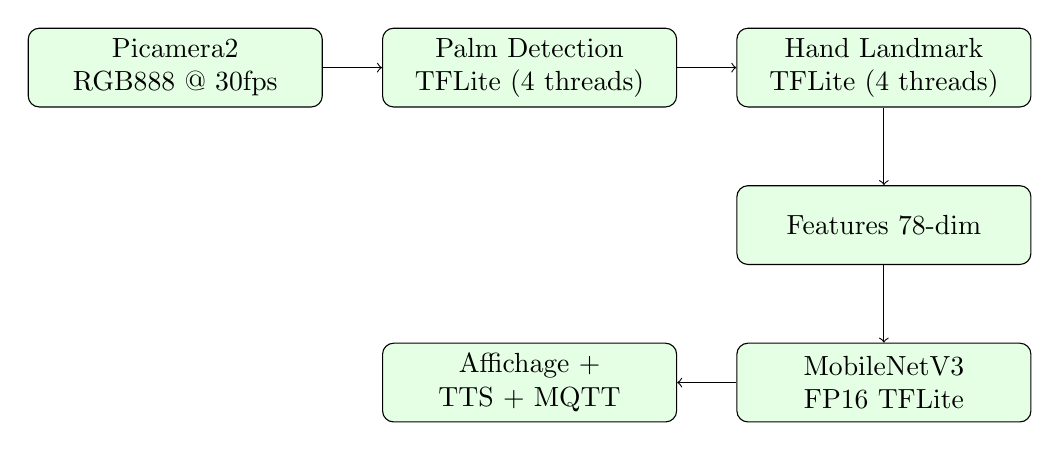
\begin{tikzpicture}[node distance=2cm, auto,
        block/.style={rectangle, draw, fill=green!10, text width=3.5cm, text centered, rounded corners, minimum height=1cm}]
        \node[block] (cam) {Picamera2\\RGB888 @ 30fps};
        \node[block, right of=cam, node distance=4.5cm] (palm) {Palm Detection\\TFLite (4 threads)};
        \node[block, right of=palm, node distance=4.5cm] (lm) {Hand Landmark\\TFLite (4 threads)};
        \node[block, below of=lm, node distance=2cm] (feat) {Features 78-dim};
        \node[block, below of=feat, node distance=2cm] (clf) {MobileNetV3\\FP16 TFLite};
        \node[block, left of=clf, node distance=4.5cm] (out) {Affichage +\\TTS + MQTT};
        \draw[->] (cam) -- (palm);
        \draw[->] (palm) -- (lm);
        \draw[->] (lm) -- (feat);
        \draw[->] (feat) -- (clf);
        \draw[->] (clf) -- (out);
    \end{tikzpicture}
    \caption{Pipeline sur Raspberry Pi 4B}
\end{figure}

\section{Installation et Configuration}

\subsection{Préparation du Système}

\begin{lstlisting}[style=python, caption={Installation des dépendances système}, language=bash]
# Mise a jour du systeme
sudo apt update && sudo apt upgrade -y

# Dependances systeme
sudo apt install -y python3-pip python3-venv \
    libopenblas-dev espeak-ng mosquitto

# Clonage du projet
git clone https://github.com/<user>/lsf-translator.git
cd lsf-translator

# Environnement virtuel
python3 -m venv venv --system-site-packages
source venv/bin/activate

# Installation des packages Python
pip install -r requirements_pi.txt
\end{lstlisting}

\subsection{Dépendances Pi}

\begin{lstlisting}[style=python, caption={requirements\_pi.txt}]
opencv-python-headless>=4.10.0
numpy>=1.26.0
scipy>=1.13.0
flask>=3.0.0
pyttsx3>=2.90
paho-mqtt>=2.1.0
picamera2>=0.3.12
ai-edge-litert>=1.0.0
\end{lstlisting}

\subsection{Runtime TFLite}

Le package \texttt{ai-edge-litert} (successeur de \texttt{tflite-runtime}) fournit l'interpréteur TFLite optimisé pour ARM64 sans nécessiter l'installation complète de TensorFlow (2+ Go) :

\begin{lstlisting}[style=python, caption={Chargement adaptatif de l'interpréteur TFLite}]
def _load_interpreter(model_path):
    try:
        from tflite_runtime.interpreter import Interpreter
        return Interpreter(model_path=model_path, num_threads=4)
    except ImportError:
        pass
    try:
        from ai_edge_litert import interpreter as litert
        return litert.Interpreter(model_path=model_path)
    except (ImportError, AttributeError):
        pass
    import tensorflow as tf
    return tf.lite.Interpreter(model_path=model_path,
                               num_threads=4)
\end{lstlisting}

\section{Optimisations Spécifiques au Pi}

\subsection{Utilisation des 4 Cœurs}

L'interpréteur TFLite est configuré avec \texttt{num\_threads=4} pour exploiter les 4 cœurs Cortex-A72 du BCM2711 :

\begin{itemize}
    \item Thread 1 : Capture caméra (producteur)
    \item Threads 2--4 : Inférence TFLite (parallélisme interne XNNPACK)
    \item Thread principal : Orchestration et affichage
\end{itemize}

\subsection{Modèle FP16}

Le modèle FP16 offre le meilleur compromis pour le Pi :
\begin{itemize}
    \item Taille réduite de 47\% par rapport à FP32 (138 Ko vs 260 Ko)
    \item Précision quasi-identique à FP32
    \item Compatible avec les opérations NEON du Cortex-A72
\end{itemize}

\subsection{Capture Native avec Picamera2}

\texttt{Picamera2} utilise le driver \texttt{libcamera} natif du Pi, offrant :
\begin{itemize}
    \item Accès direct au capteur Sony IMX219 sans conversion
    \item Format RGB888 natif (pas de conversion BGR$\rightarrow$RGB nécessaire)
    \item Contrôle précis du framerate et de l'exposition
    \item Latence réduite par rapport à OpenCV + V4L2
\end{itemize}

\section{Accès Distant}

Le serveur Flask MJPEG permet d'accéder au flux vidéo annoté depuis n'importe quel appareil sur le réseau local :

\begin{verbatim}
http://<IP_DU_PI>:5000/stream
\end{verbatim}

Cela permet de visualiser la traduction en temps réel sur un smartphone, une tablette ou un PC distant sans installer de logiciel supplémentaire.

\section{Exécution}

\begin{lstlisting}[style=python, caption={Lancement sur Raspberry Pi}, language=bash]
cd ~/lsf_translator
source venv/bin/activate
python3 main_pi.py
\end{lstlisting}

Le système démarre et affiche :
\begin{verbatim}
[Pi] Model loaded: models/static_mobilenetv3_fp16.tflite
[Pi] Running... Press Ctrl+C to stop.
[Pi] Stream at http://<PI_IP>:5000/stream
\end{verbatim}
